\documentclass{beamer}
\usetheme{Boadilla}
\usepackage{thumbpdf}
\usepackage{wasysym}
\usepackage{ucs}
\usepackage[utf8]{inputenc}
\usepackage{pgf,pgfarrows,pgfnodes,pgfautomata,pgfheaps,pgfshade}
\usepackage{verbatim}
\usepackage{listings}
\usepackage{color}
\begin{document}

\setbeamertemplate{navigation symbols}{%

}

\pdfinfo
    {
      /Title       (Formation Git)
      /Creator     (Tex)
      /Author      (Nicolas Aguirre)
      /Date        (26 Mars 2013)
    }


    \title{Formation GIT}
    \subtitle{Logiciel de gestion de version décentralisé}
    \author{Nicolas Aguirre}
    \date{26 Mars 2013}

    \frame{\titlepage}
%-------------------------------------------------------------------------------
    \begin{frame}\frametitle{Plan}
      \tableofcontents
    \end{frame}
  %-------------------------------------------------------------------------------

    \section{Présentation de Git}

    \begin{frame}
      \frametitle{Définition de GIT}
      \begin{itemize}
        \item Logiciel de gestion de version décentralisé
        \item Permet de stocker un ensemble de fichiers en conservant la chronologie des modifications
        \item Permet de stocker l'ensemble des modifications et des relations localement sans avoir à se connecter à un serveur.
      \end{itemize}
    \end{frame}

    \begin{frame}
      \frametitle{Historique}
      \begin{itemize}
      \item Projet initié par Linus Torvalds pour le noyau linux.
      \item Première version le 7 Avril 2005.
      \item Logiciel de gestion de versions decentralisé.
      \item Semblable à Mercurial ou Bitkeeper.
      \item Version actuelle 1.8.0
      \item Licence GPLv2.
      \item http://git-scm.com
      \end{itemize}
    \end{frame}

    \begin{frame}
      \frametitle{Git vs SVN}
      \begin{itemize}
        \item GIT != SVN.
        \item Ne jamais se demander quelle est la version SVN de cette commande.
        \item svn checkout != git checkout.
        \item Dans svn trunk est LA branche.
        \item Dans git master est UNE branche parmis d'autres.
      \end{itemize}
    \end{frame}

%-------------------------------------------------------------------------------
    \section{Notions de Workflows}
    \begin{frame}
      \frametitle{Workflows}
      \begin{itemize}
        \item Un workflow est un ensemble de tâches et d'opérations effectuées par:
          \begin{itemize}
            \item Un développeur;
            \item Un intégrateur;
            \item Une société;
          \end{itemize}
      \end{itemize}
    \end{frame}
    \begin{frame}
      \frametitle{Workflow développeur}
      \begin{itemize}
        \item Créer une branche de dev.
        \item Commiter comme bon vous semble.
        \item Aussi souvent que vous voulez.
        \item Pusher ou merger les commits en ensembles cohérents.
      \end{itemize}
    \end{frame}

    \begin{frame}
      \frametitle{Workflow développeur}
      \begin{itemize}
        \item Supprime la peur de ne pas être à jour.
        \item Permet de faire de la revue de code sur des ensembles cohérents.
        \item Permet de travailler par fonctionnalitées.
        \item Permet d'expérimenter dans des branches.
        \item Le développeur devient un producteur de code source.
      \end{itemize}
    \end{frame}

    \begin{frame}
      \frametitle{Workflow de l'intégrateur}
      \begin{itemize}
        \item Récupération des commits dans une branche.
        \item Intégration par fonctionalités.
        \item Test des fonctionalités.
        \item Génération de branche par livraison.
        \item Génération de tags.
      \end{itemize}
    \end{frame}

    \begin{frame}
      \frametitle{Workflow de la société}
      \begin{itemize}
        \item Utilisation d'un serveur de référence.
        \item Possibilité de stocker toutes les branches des développeurs et des intégrateurs.
        \item Possibiltié de stocker uniquement les branches livrées.
      \end{itemize}
    \end{frame}
%-------------------------------------------------------------------------------
    \section{Base de données GIT}

    \begin{frame}
      \frametitle{Répertoire .git}
      \begin{itemize}
      \item La base de donnée est stockée dans le répertoire .git à la racine de votre projet.
      \end{itemize}
    \end{frame}

    \begin{frame}
      \frametitle{Comment sont stockées les données dans SVN}
      \begin{itemize}
        \item Dans SVN l'information d'un commit est stockée sous forme de différences:
          \begin{center}
            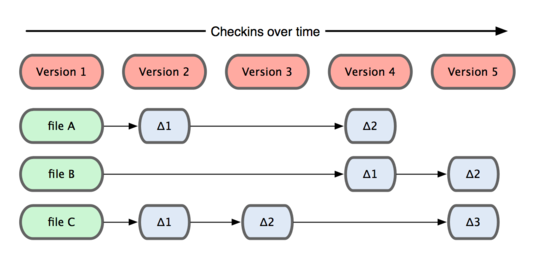
\includegraphics[width=8cm]{imgs/deltas.eps}
          \end{center}
      \end{itemize}
    \end{frame}

   \begin{frame}
      \frametitle{Comment sont stockées les données dans GIT}
      \begin{itemize}
        \item Git fait un snapshot des fichiers a chaque version:
          \begin{center}
            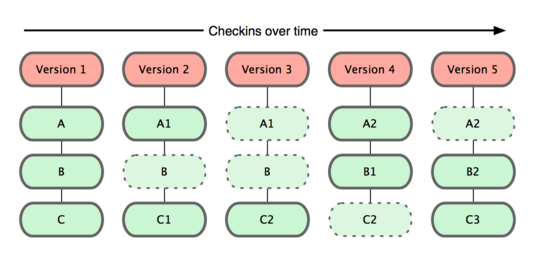
\includegraphics[width=8cm]{imgs/snapshot.eps}
          \end{center}
      \end{itemize}
    \end{frame}

    \begin{frame}
      \frametitle{Comment sont stockées les données dans GIT}
      \begin{itemize}
      \item Git indexe les fichiers d'après leur somme de contrôle SHA1.
      \item Les fichiers sont donc stockés uniquement si ils sont modifiés.
      \item Si un fichier est modifié il est stocké deux fois sur le disque.
      \end{itemize}
    \end{frame}

   \begin{frame}
      \frametitle{Toutes les informations sont stockées en local}
      \begin{itemize}
        \item Toutes les informations sont stockées en local sur votre disque.
        \item Pas de latence due au réseau.
        \item L'historique de tout le projet est local.
        \item Toutes les objets git ont une somme de contrôle SHA-1.
      \end{itemize}
    \end{frame}
%-------------------------------------------------------------------------------
   \section{Les 3 zones}

   \begin{frame}
     \frametitle{Les 3 zones}
     \begin{itemize}
     \item la zone ``working directory''
     \item la zone ``staging area''
     \item la zone ``git directory(repository)''
     \end{itemize}
   \end{frame}

  \begin{frame}
     \frametitle{Les 3 zones}
     \begin{center}
       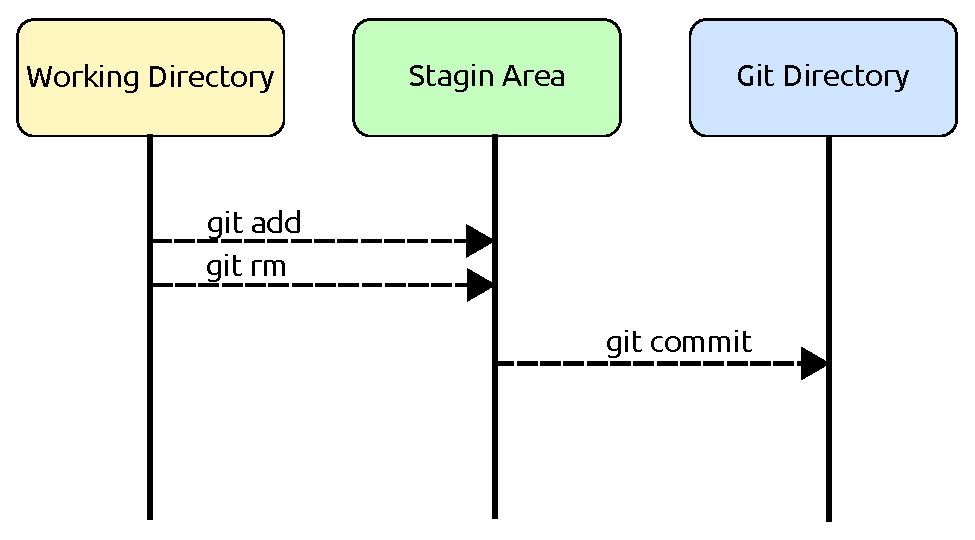
\includegraphics[width=11cm]{imgs/3zones.eps}
     \end{center}
  \end{frame}

  \begin{frame}
     \frametitle{Git directory}
     \begin{itemize}
     \item C'est ce qui est copié lorsque vous clonez un dépôt d'un autre endroit.
     \item C'est la base de donnée de git.
     \item C'est l'endroit où il stocke tous les commits, et toutes les relations entre commits.
     \end{itemize}
   \end{frame}

  \begin{frame}
     \frametitle{Working directory}
     \begin{itemize}
     \item C'est un snapshot d'une des version du projet.
     \item Les fichiers sont issues de la base de données du git directory.
     \item Git les place sur le disque pour que vous puissiez les utiliser ou les modifier.
     \end{itemize}
   \end{frame}

  \begin{frame}
     \frametitle{Staging Area}
     \begin{itemize}
     \item C'est un fichier qui contient les informations de ce qui ira dans votre prochain commit.
     \end{itemize}
   \end{frame}

%-------------------------------------------------------------------------------

\section{Commandes de base}

  \begin{frame}
     \frametitle{Mon premier commit}
     \begin{center}
       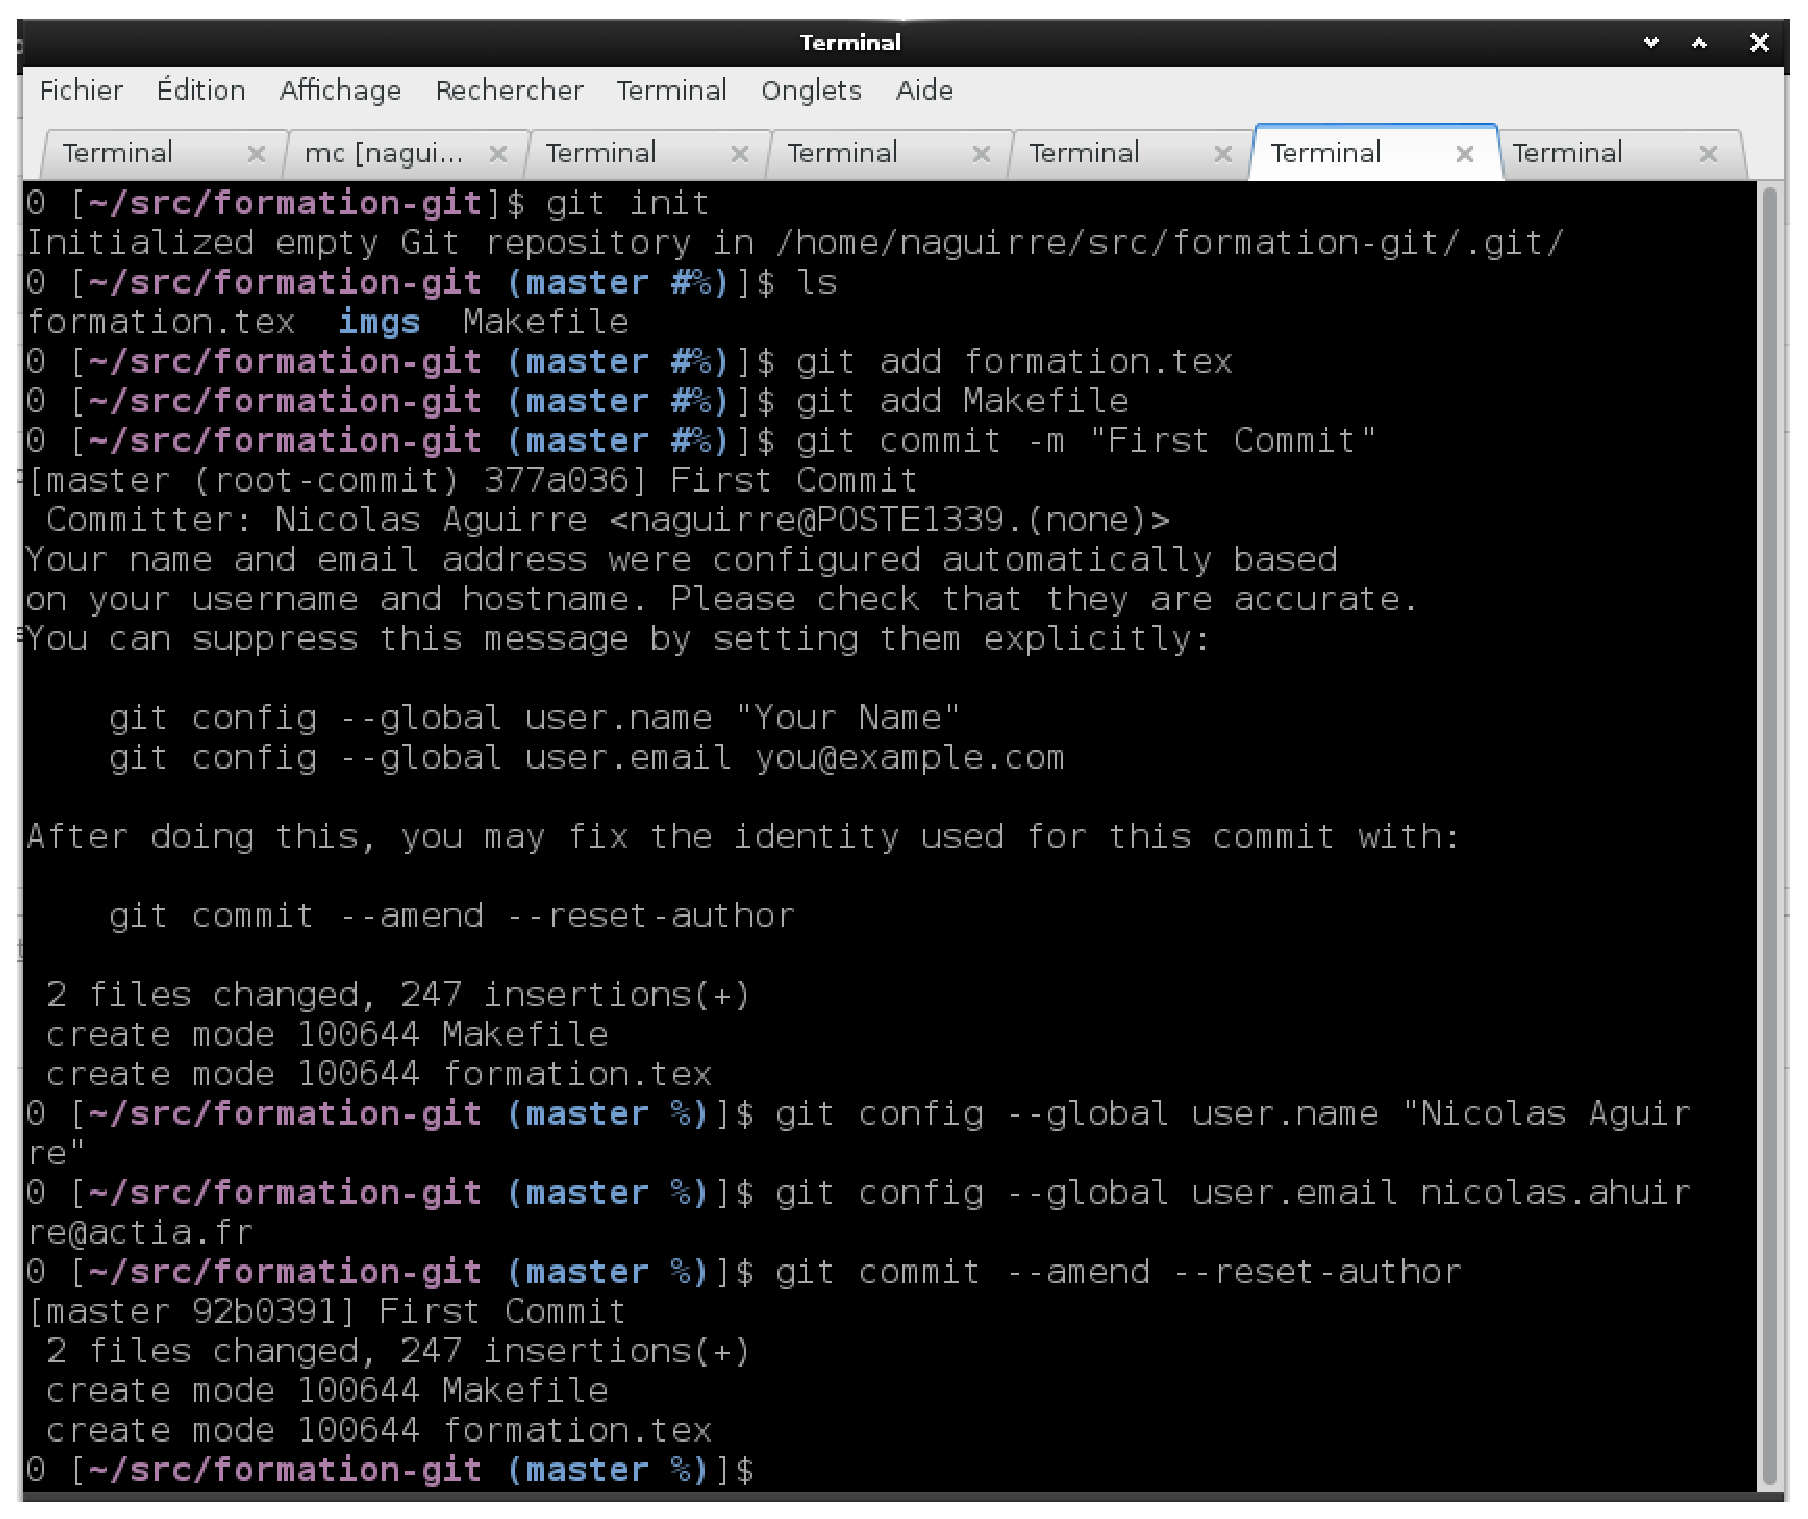
\includegraphics[width=9cm]{imgs/first_commit.eps}
     \end{center}
  \end{frame}

  \begin{frame}
     \frametitle{git status}
     \begin{center}
       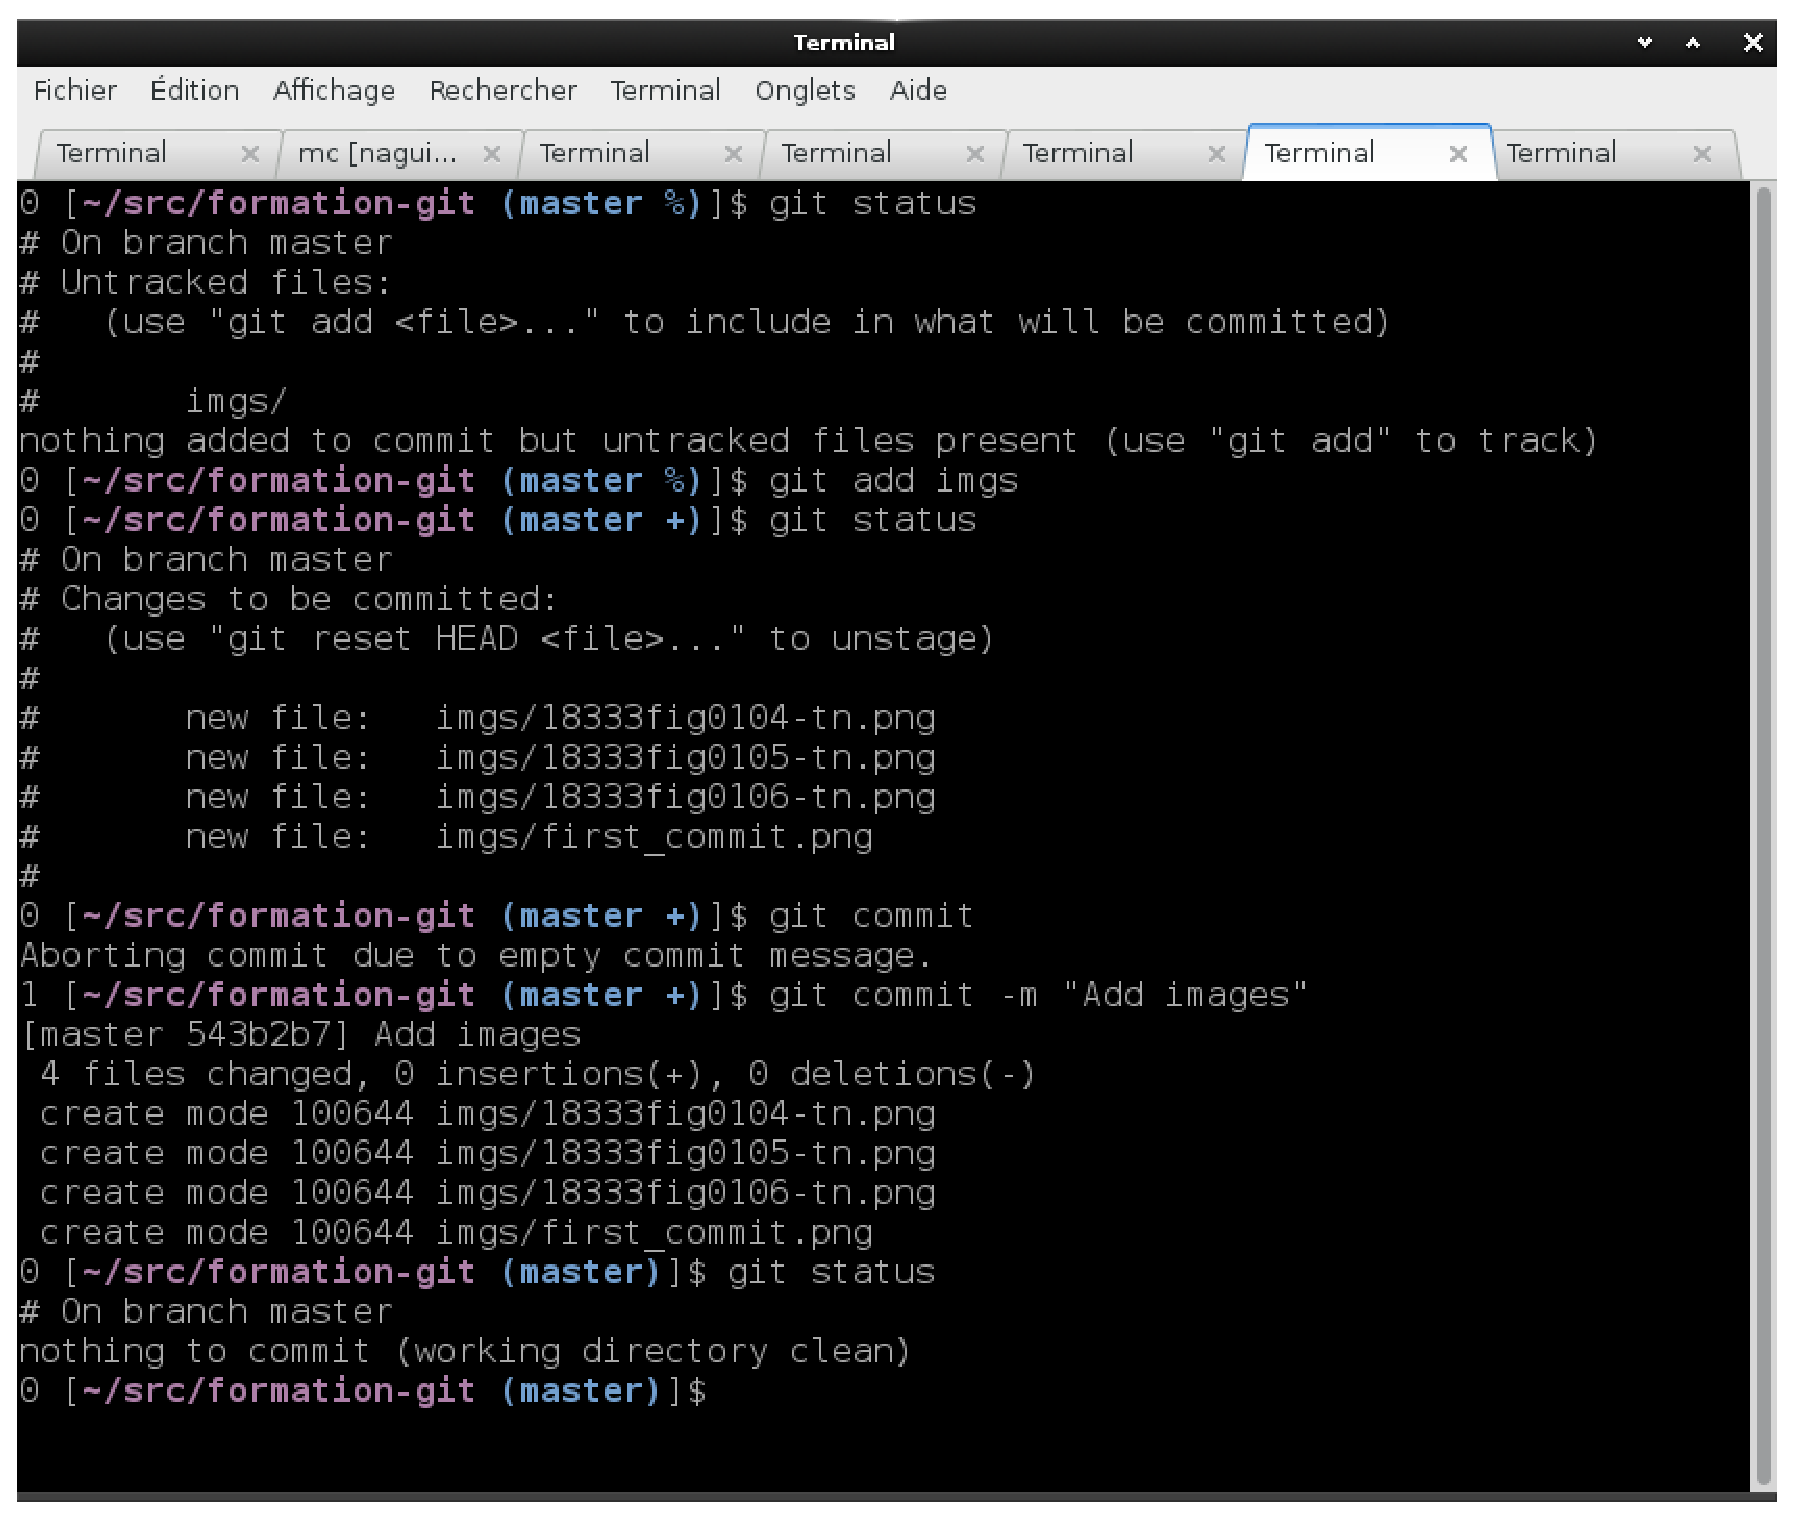
\includegraphics[width=9cm]{imgs/status.eps}
     \end{center}
  \end{frame}

\begin{frame}[fragile]\frametitle{Visualisation}
  Historique des commits: \verb|git log|

  \begin{semiverbatim}
  \$ \alert{git log}
  \end{semiverbatim}

  Visualisation des différences: \verb|git diff et git diff --staged|
  \begin{semiverbatim}
  \$ \alert{git diff}
  \$ \alert{git diff --staged}
  \end{semiverbatim}

\end{frame}

\begin{frame}[fragile]
  \frametitle{Récapitulatif des commandes de base}
  \begin{semiverbatim}
    \$ git init
    \$ git add
    \$ git rm
    \$ git commit
    \$ git status
    \$ git diff
    \$ git log
    \$ git tag
    \$ git branch
    \$ git checkout
  \end{semiverbatim}
\end{frame}

\begin{frame}
  \frametitle{Outil graphique: gitg, gitk, git gui}
  \begin{itemize}
  \item gitg et gitk sont des outils graphique permettant de visualiser plus facilement l'arbre de commits.
  \item git gui est un outil graphique permettant de commiter de maniére graphique.
  \item il existe egalement Tortoise git sur windows
  \end{itemize}
\end{frame}

%-------------------------------------------------------------------------------

\section{Travailler avec des serveurs distants}
\begin{frame}
  \frametitle{Buildroot}
  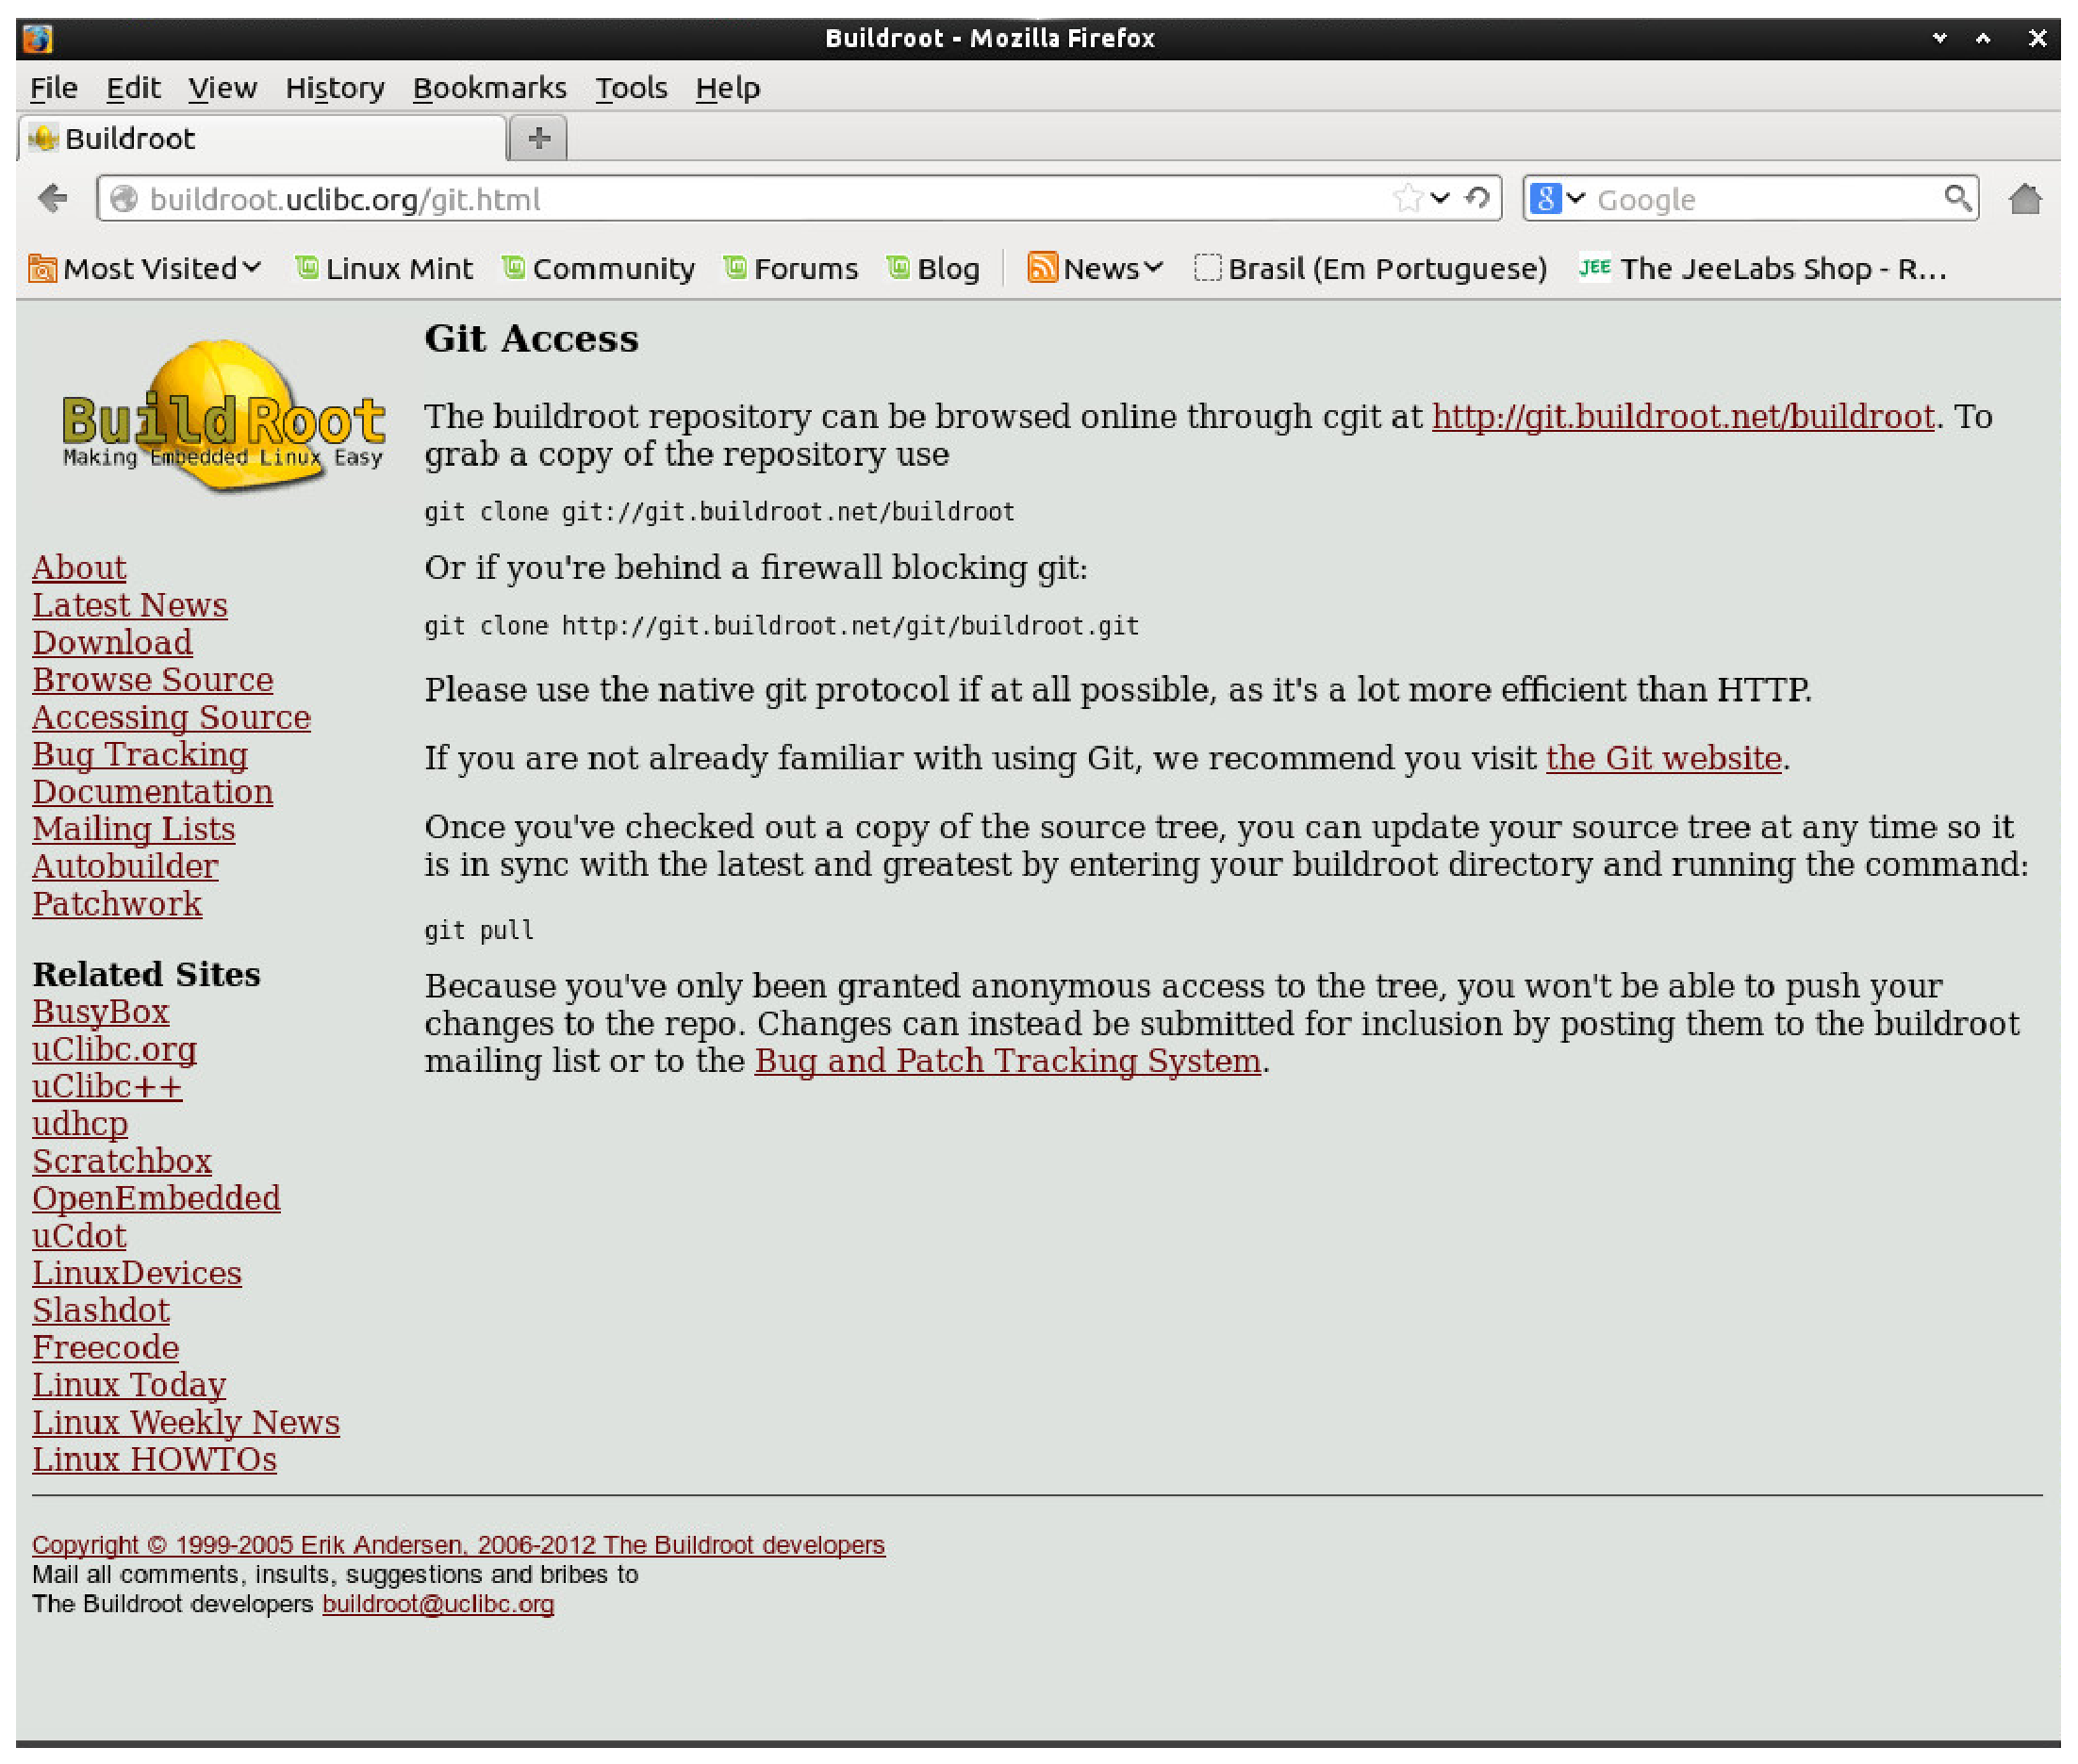
\includegraphics[width=9cm]{imgs/buildroot.eps}
\end{frame}


\begin{frame}
  \frametitle{git clone}
  \begin{semiverbatim}
    \$ git clone http://git.buildroot.net/git/buildroot.git
  \end{semiverbatim}
  \begin{itemize}
    \item Permet de copier à l'identique le dépot distant sur sa machine.
    \item Les tags, branches et l'intégralité de tous les commits sont récupérés.
  \end{itemize}
\end {frame}

\begin{frame}
  \frametitle{Seveurs distants}
  \begin{semiverbatim}
    \$ git remote -v

    origin git://git.buildroot.net/buildroot (fetch)

    origin git://git.buildroot.net/buildroot (push)
  \end{semiverbatim}
\end{frame}

\begin{frame}
  \frametitle{Récapitulatif des commandes}
  \begin{itemize}
  \item push : action d'envoyer les commits ainsi que les relations entre commits vers le serveur distant (origin par défaut).
  \item fetch : action de récupérer les commits ainsi que les relations entre commits depuis le serveur distant.
  \end{itemize}
\end{frame}

\begin{frame}
  \frametitle{Ajout d'un serveur}
  \begin{semiverbatim}
    \$ git remote add forge3 git@forge3:buildroot

    \$ git remote -v

    origin git@forge3:buildroot (fetch)

    origin git@forge3:buildroot (push)

  \end{semiverbatim}
\end{frame}

\begin{frame}
  \frametitle{Checkout}
  \begin{semiverbatim}
    \$ git checkout (tag ou sha1 ou branch)
    
    Git présente sur le systeme de fichier la version qu'on lui demande.
  \end{semiverbatim}
\end{frame}

\begin{frame}
  \frametitle{Pull/Push}
  \begin{semiverbatim}
    \$ git pull

    \$ git pull --rebase
  \end{semiverbatim}
  \begin{itemize}
  \item Git récupère les commits distant et merge la branche actuelle avec la branche distante.
  \item Par défaut git merge les branches lors d'un pull.
  \item Rebase la branche actuelle avec la branche distante.
  \end{itemize}
\end{frame}

\begin{frame}
\frametitle{Merge/Rebase}
    \begin{center}
     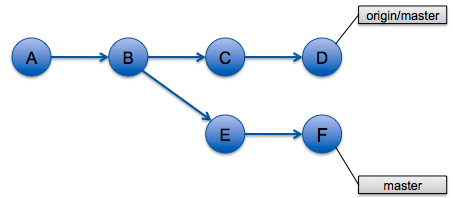
\includegraphics[width=11cm]{imgs/before-merge.png}
     \end{center}
\end{frame}

\begin{frame}
\frametitle{Merge/Rebase}
    \begin{center}
     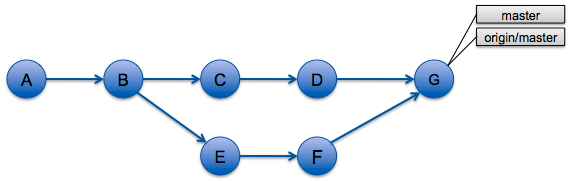
\includegraphics[width=11cm]{imgs/git-merge2.png}
     \end{center}
\end{frame}

\begin{frame}
\frametitle{Merge/Rebase}
    \begin{center}
     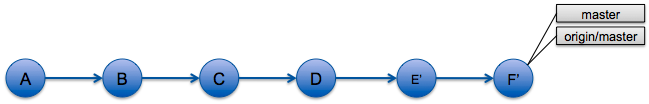
\includegraphics[width=11cm]{imgs/git-rebase.png}
     \end{center}
\end{frame}

%-------------------------------------------------------------------------------

\section{Commandes avancées}
\begin{frame}
  \frametitle{Pour aller plus loin}
  \begin{semiverbatim}
    \$ git stash

    \$ git reflog

    \$ git reset
  \end{semiverbatim}
\end{frame}

\section{Credits}
\begin{frame}
  \frametitle{Credits}
  \begin{itemize}
  \item http://blog.octo.com/git-dans-la-pratique-22/
  \item pour récupérer la formation:
  \item git clone https://github.com/naguirre/formation-git.git
  \end{itemize}
  
\end{frame}

\end{document}
